%-------------------------
% Resume in Latex
% Based off of: https://github.com/sb2nov/resume
% and Jake Gutierrez's version of it
% at https://www.overleaf.com/latex/templates/jakes-resume/syzfjbzwjncs
% inspired by https://practicaltypography.com/resumes.html
% License : MIT
%------------------------

\documentclass[a4paper,11pt]{article}

\usepackage{latexsym}
\usepackage[empty]{fullpage}
\usepackage{titlesec}
\usepackage{marvosym}
\usepackage[usenames,dvipsnames]{xcolor}
\usepackage{verbatim}
\usepackage{enumitem}
\usepackage[hidelinks]{hyperref}
\usepackage[margin = 1in]{geometry}
\usepackage{fancyhdr}
\usepackage[english]{babel}
\usepackage{tabularx}
\usepackage{wrapfig}
\usepackage{graphicx}

%--------------UNDERLINING---------------
% taken from https://alexwlchan.net/2017/10/latex-underlines/

\usepackage{contour}
\usepackage{ulem}

\renewcommand{\ULdepth}{3.8pt}
\contourlength{0.8pt}

\newcommand{\myuline}[1]{%
  \uline{\phantom{#1}}%
  \llap{\contour{white}{#1}}%
}

%----------------------------------------

\graphicspath{ {./Images/} }

%----------FONT OPTIONS----------
\usepackage{fontspec}
\usepackage{fontawesome5}

% I could have just used the charter package here for the font I wanted...
% but I'd still need to change compiler to XeLaTeX to include the title font
% \usepackage{charter}

\setmainfont{XCharter}

\newfontfamily{\basictitle}{basictitlefont}[
Path = Fonts/,
Extension = .ttf,
UprightFont = basictitlefont
]
% to use:
% {\basictitle This text uses the basictitle font}

\pagestyle{fancy}
\fancyhf{} % clear all header and footer fields
\fancyfoot{}
\renewcommand{\headrulewidth}{0pt}
\renewcommand{\footrulewidth}{0pt}

% Adjust margins
\iffalse
% \iftrue
\addtolength{\oddsidemargin}{0.3in}
\addtolength{\marginparsep}{0.3in}
\addtolength{\evensidemargin}{0.3in}
\addtolength{\textwidth}{-0.5in}
\addtolength{\topmargin}{0.3in}
\addtolength{\textheight}{0.3in}
\fi

\urlstyle{same}

\raggedright
\setlength{\tabcolsep}{0in}

% Sections formatting
\titleformat{\section}{
    {\color{gray}\titlerule} \vspace{-5pt}
    \vspace{8pt}\scshape\raggedright\normalfont
}{}{0pt}{}

%-------------------------
% Custom commands
\newcommand{\resumeItem}[1]{
  \item\small{
    {#1 \vspace{-2pt}}
  }
}

\newcommand{\resumeSubheading}[4]{
  \vspace{-2pt}\item
    \begin{tabular*}{0.97\textwidth}[t]{l@{\extracolsep{\fill}}r}
      \textbf{#1} & #2 \\
      \textit{\small#3} & \textit{\small #4} \\
    \end{tabular*}\vspace{-7pt}
}

\newcommand{\resumeSubSubheading}[2]{
    \item
    \begin{tabular*}{0.97\textwidth}{l@{\extracolsep{\fill}}r}
      \textit{\small#1} & \textit{\small #2} \\
    \end{tabular*}\vspace{-7pt}
}

\newcommand{\resumeProjectHeading}[2]{
    \item
    \begin{tabular*}{0.97\textwidth}{l@{\extracolsep{\fill}}r}
      \small#1 & #2 \\
    \end{tabular*}\vspace{-7pt}
}

\newcommand{\resumeSubItem}[1]{\resumeItem{#1}\vspace{-4pt}}

\renewcommand\labelitemii{$\vcenter{\hbox{\tiny$\bullet$}}$}

\newcommand{\resumeSubHeadingListStart}{\begin{itemize}[leftmargin=0.15in, label={}]}
\newcommand{\resumeSubHeadingListEnd}{\end{itemize}}
\newcommand{\resumeItemListStart}{\begin{itemize}}
\newcommand{\resumeItemListEnd}{\end{itemize}\vspace{-5pt}}

%-------------------------------------------
%%%%%%  RESUME STARTS HERE  %%%%%%%%%%%%%%%%%%%%%%%%%%%%


\begin{document}

% ----- TOGGLE PHOTO --------
% comment out \iffalse and remove the % from \iftrue to toggle photo
\iffalse
% \iftrue
\begin{wrapfigure}{R}{0.15\textwidth}
\vspace{-35pt}
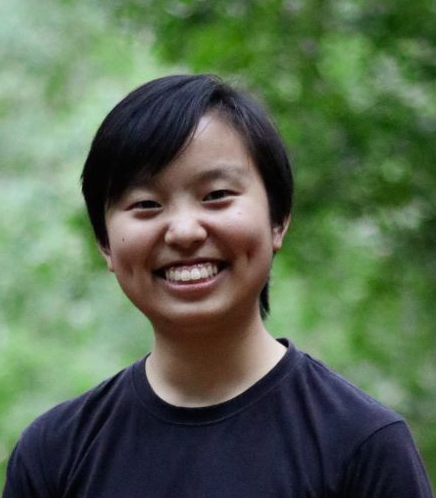
\includegraphics[scale=0.20]{dp_cropped}
\end{wrapfigure}
\fi

%----------HEADING----------

{\basictitle \Huge Rateeb Riyasat}
\\

% ----- TOGGLE FOR PHOTO ----
% \vspace{10pt}

\href{mailto:rateebriyasat@ufl.edu}{
    \faEnvelope
    \thinspace \thinspace
    \myuline{rateebriyasat@ufl.edu}} $|$
\href{https://github.com/bmollusk}{
    \faGithub
    \thinspace \thinspace
    \myuline{bmollusk}} $|$
\faPhone
\thinspace \thinspace
+1 561 334 8916

%-----------EDUCATION-----------
\section{Education}
  \resumeSubHeadingListStart
    \resumeSubheading
      {University of Florida}{Gainesville, Florida}
      {Bachelors of Science in Computer Science, Mathematics}{May 2024}
      \resumeItemListStart
      
        \resumeItem{GPA: 3.64/4.0}
        
        \resumeItem{Relevant Coursework: Discrete Structures(current), Programming Fundamentals, Engineering Statistics, Combinatorics(self-taught)}

      \resumeItemListEnd
      
  \resumeSubHeadingListEnd
  
    %-----------PROJECTS-----------
\section{Coding Projects}
    \resumeSubHeadingListStart
      \resumeProjectHeading
          {\href{https://github.com/bmollusk/stickiernotes}{\myuline{\textbf{StickierNotes}}} $|$ \textit{Python,PyQt5,QMake}}{Sept 2020 -- Present}
          \resumeItemListStart
            \resumeItem{Designed easy to read minimal graphical interface to permit seamless integration into the users workflow}
            \resumeItem{Opened possibilities for rapid development of new user-created commands with easy to use framework}
            \resumeItem{Implemented robust and meticulous reference system to allow for easy referencing of prior calculations}
          \resumeItemListEnd
    \resumeProjectHeading
          {\href{https://github.com/bmollusk/croptool}{\myuline{\textbf{bbCropTool}}} $|$ \textit{C++,Qt5,QMake}}{July -- Aug 2020}
          \resumeItemListStart
            \resumeItem{Utilized Qt5 to set up custom UI system that adapts to aspect ratio changes for both the app content and the imported file}
            \resumeItem{Built robust system for saving preset cropping layouts as files to be loaded in later to allow for easy integration into an existing pipeline}
            \resumeItem{Made intelligent auto-adapting slider framework to allow for easy adjustments to lower the learning curve required to easily adopt the utility in a team setting}
          \resumeItemListEnd
    \resumeSubHeadingListEnd


%-----------EXPERIENCE-----------
\section{Experience}
  \resumeSubHeadingListStart
  
    \resumeSubheading
      {Marketing Committee}{October 2020 -- Present}
      {University of Florida SASE South Regional Conference Planning Committee}{Remote}
      \resumeItemListStart
        \resumeItem{Coordinated strategies to garner more participation before and during the event, garnering over 100+ applicants during the first couple weeks alone}
      \resumeItemListEnd

    \resumeSubheading
      {Visiting Researcher}{Jun -- July 2019}
      {University of Tokyo}{Tokyo, Japan}
      \resumeItemListStart
        \resumeItem{Proposed novel video prediction method utilizing Convolutional Long-Short Term Memory paired with an Artificial Neural Network based Voting System}
        \resumeItem{Oversaw the building of a remote GPU Farm for rapid and easy training and evaluation of Machine Learning Models}
        \resumeItem{Utilized Pytorch and Numpy to rapidly develop an initial prototype of the model for initial testing and further development}
      \resumeItemListEnd
      
  \resumeSubHeadingListEnd
%-----------ACHIEVEMENTS-----------
\section{Achievements}
\resumeSubHeadingListStart
    \resumeSubheading
      {Top 19\% of Papers}{March 2020}
      {Team14057}{M3 Mathworks Math Modeling Challenge}
  \resumeSubHeadingListEnd
%-----------PROGRAMMING SKILLS-----------
\section{Skills}
 \begin{itemize}[leftmargin=0.15in, label={}]
    \small{\item{
     \textbf{Languages}{: Python, C/C++, SQL, JavaScript, HTML/CSS, R, MATLAB} \\
     \textbf{Frameworks}{: Pytorch, PyQt5, Qt4/5, NodeJS, SQLite} \\
     \textbf{Developer Tools}{: Jupyter Notebooks, Git, VS Code, Bash, LaTEX} \\
     }
     }
 \end{itemize}

%-------------------------------------------
\end{document}
